\documentclass{standalone}

\usepackage{tikz}

\usetikzlibrary{positioning, shadows, fit, arrows.meta, backgrounds}

\begin{document}

\begin{tikzpicture}[node distance=0.5cm, pipestep/.style={fill=white, draw, rectangle, drop shadow, minimum width=5cm}]
	\node[label={ADNI Dataset}, pipestep] (adni) {T1-weighted MRI ($N=443$)};

	\node[below=of adni, inner sep=0] (skull) {skull stripping};
	\node[below=0.5em of skull, inner sep=0] (gms) {gray matter segmentation};
	\node[below=0.5em of gms, inner sep=0] (im_reg) {non-linear registration};

	\begin{scope}[on background layer]
		\node[fit=(skull)(gms)(im_reg), pipestep] (pre) {};
	\end{scope}
	\node[rotate=90, left=of pre, anchor=center] {Pre-Processing};

	\draw[-latex] (adni.south) -- (pre.north);

	\node[label={[name=cn_label]below:{$CN = 254$}}, xshift=-1.25cm, below=of pre] (cn) {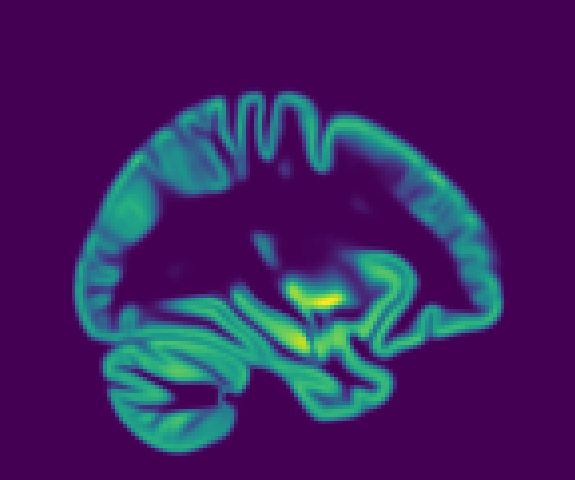
\includegraphics[width=2cm]{figures/cn_slice.png}};

	\node[label={[name=ad_label]below:{$AD = 189$}}, xscale=-1, xshift=-1.25cm, below=of pre] (ad) {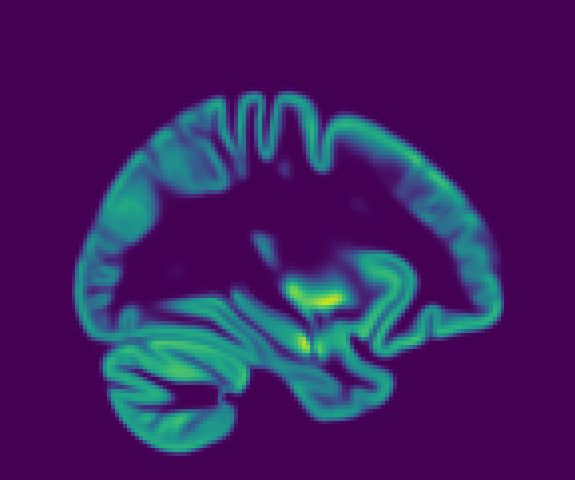
\includegraphics[width=2cm]{figures/ad_slice.png}};


	\begin{scope}[on background layer]
		\node[fit=(ad)(ad_label)(cn)(cn_label), pipestep] (data) {};
	\end{scope}

	\draw[-latex] (pre.south) -- (data.north);
\end{tikzpicture}

\end{document}
